\documentclass{beamer}
\usepackage{graphicx}
%\usepackage{xcolor}
\usepackage{color}
\usepackage{transparent}
\usepackage{setspace}
%\usepackage{enumitem}
%\setlist[itemize]{leftmargin=*}
\newcommand{\figpath}{../../Figures/}
\newcommand{\red} [1]{\textcolor{red}{#1}}
\newcommand{\blue}[1]{\textcolor{blue}{#1}}
\newcommand{\black}[1]{\textcolor{black}{#1}}
%\newcommand{\green}[1]{\textcolor{green}{#1}}
\newcommand{\green}[1]{\textcolor{yellow}{#1}}
\newcommand{\yellow}[1]{\textcolor{yellow}{#1}}
\newcommand{\slidecite}[3]{[{\sc {#1},{\it {#2}}{#3}}]}
\newcommand{\pdf}{\operatorname{pdf}}

%-------------- aliases -----------------------
\newcommand{\ie}{{\it i.e.\,}}
\newcommand{\vs}{{\it vs.\,}}
\newcommand{\eg}{{\it e.g.\,}}
\newcommand{\abinitio}{{\it ab initio} }
\newcommand{\nablab}{{\boldsymbol{\nabla}}}
\newcommand{\Upsilonb}{{\boldsymbol{\Upsilon}}}
\newcommand{\Ab}{\mathbf{A}}
\newcommand{\As}{\mathsf{A}}
\newcommand{\Bc}{\mathcal{B}}
\newcommand{\ab}{\mathbf{a}}
\newcommand{\db}{\mathbf{d}}
\newcommand{\eb}{\mathbf{e}}
\newcommand{\fb}{\mathbf{f}}
\newcommand{\Ep}{\mathbb{E}}
\newcommand{\yb}{\mathbf{y}}
\newcommand{\dx}{\Delta\mathbf{x}}
\newcommand{\xb}{\mathbf{x}}
\newcommand{\rb}{\mathbf{r}}
\newcommand{\pb}{\mathbf{p}}
\newcommand{\Xb}{\mathbf{X}}
\newcommand{\Xs}{\mathsf{X}}
\newcommand{\Rb}{\mathbf{R}}
\newcommand{\cluster}{\mathcal{C}}
\newcommand{\Ib}{\mathbf{I}}
\newcommand{\Is}{\mathsf{I}}
\newcommand{\Pb}{\mathbf{P}}
\newcommand{\Ps}{\mathsf{P}}
\newcommand{\Pp}{\mathbb{P}}
\newcommand{\Ub}{\mathbf{U}}
\newcommand{\Us}{\mathsf{U}}
\newcommand{\Vb}{\mathbf{V}}
\newcommand{\Vs}{\mathsf{V}}
\newcommand{\Ws}{\mathsf{W}}
\newcommand{\Db}{\mathbf{D}}
\newcommand{\Ds}{\mathsf{D}}
\newcommand{\Sb}{\mathbf{S}}
\newcommand{\Mb}{\mathbf{M}}
\newcommand{\spn}{\operatorname{span}}
\newcommand{\tr}{\operatorname{tr}}
\newcommand{\RMSD}{\operatorname{RMSD}}
\newcommand{\SVD}{\operatorname{SVD}}
\newcommand{\Ball}{\mathcal{B}}
\newcommand{\argmin}{\operatorname{argmin}}
\newcommand{\argmax}{\operatorname{argmax}}


\begin{document}
\title{
\red{\underline{\tiny 13$^\text{th}$ U.S. National Congress on Computational Mechanics, San Diego, July 26-30, 2015}} \\
{\bf Smart use of Density Functional Theory calculations to drive Newtonian dynamics} \\
\vspace{-0.1in}
{\tiny \it Concurrent Multi-length Scale Modeling: From Finite Elements to Atoms and Electrons} \\
\vspace{-0.1in}
{\tiny Monday. 4:30pm } \\
\vspace{-0.01in}
\large
\black{{\bf Reese Jones} and Mickey Shaughnessy} \\
\vspace{-0.01in}
\black{\it \small  Sandia National Laboratories}
\vspace{-0.1in}
\begin{center}
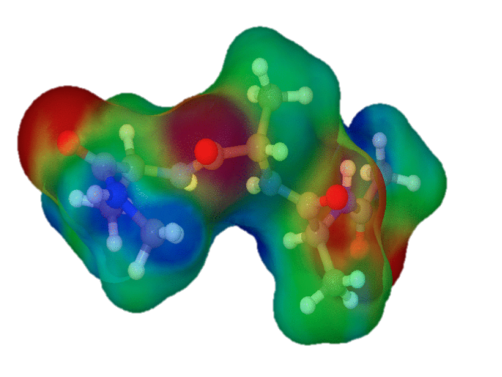
\includegraphics[width=0.5\textwidth]{\figpath/molecule_forces.pdf} \\
\fbox{
\begin{minipage}[h!]{0.85\textwidth}
\begin{spacing}{0.5}
{\tiny
Sandia National Laboratories is a multi­‐program laboratory managed and operated by Sandia Corporation, a wholly owned subsidiary of Lockheed Martin Corporation, for  the U.S. Department of Energy's  National Nuclear Security Administration  under  contract DE-­‐AC04-­‐94AL85000. }
\end{spacing}
\vspace{0.1in}
\end{minipage}
}
\end{center}
\date{}
}
%%%%%%%%%%%%%%%%%%%%%%%%%%%%%%%%%%%%%%%%%%%%%%%%%%%%%%%%%%%%%%%%%%%%%%%%%%%%
\frame{\titlepage}
%%%%%%%%%%%%%%%%%%%%%%%%%%%%%%%%%%%%%%%%%%%%%%%%%%%%%%%%%%%%%%%%%%%%%%%%%%%%
\frame{\frametitle{Outline}
\begin{minipage}[h!]{0.65\textwidth}

{\bf Motivation:}
\red{\it compositionally} and \red{\it structurally complex} materials and processes: e.g. deposition and radiation damage, require the dynamic simulation of \red{\it large} atomic systems with \red{\it multiple} interspecies interactions.

\begin{center}

\fbox{
{\bf Outline:}

\vspace{0.1in}
\begin{minipage}[h!]{0.7\textwidth}

\tableofcontents
\end{minipage}
}
\end{center}

\begin{center}
\red{please ask questions}
\end{center}
\end{minipage}\hfill%
\begin{minipage}[h!]{0.30\textwidth}
\begin{center}

atomic deposition
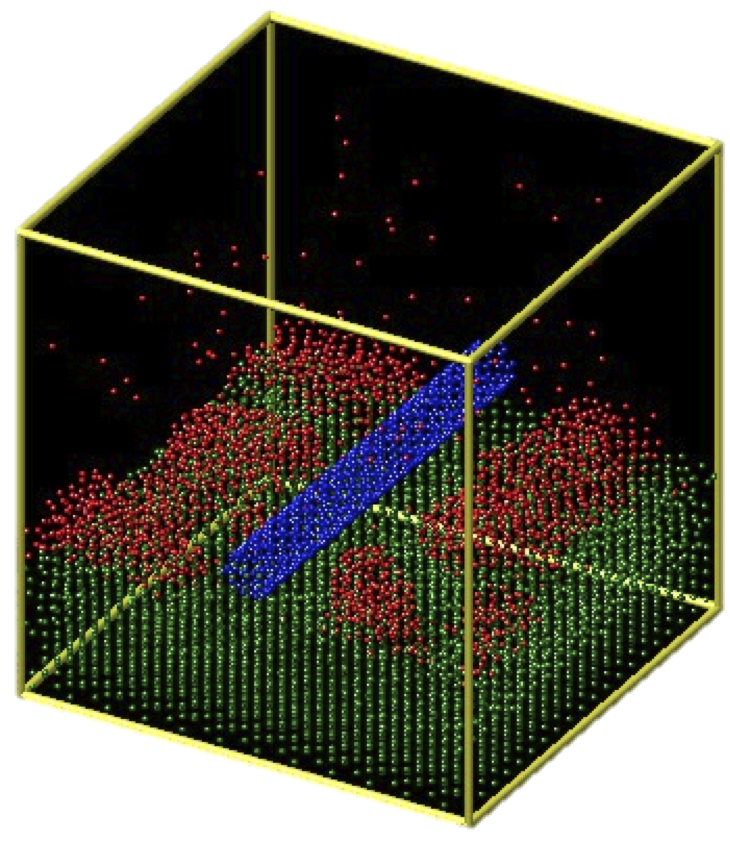
\includegraphics[width=0.95\textwidth]{\figpath/deposit.png} 

radiation damage
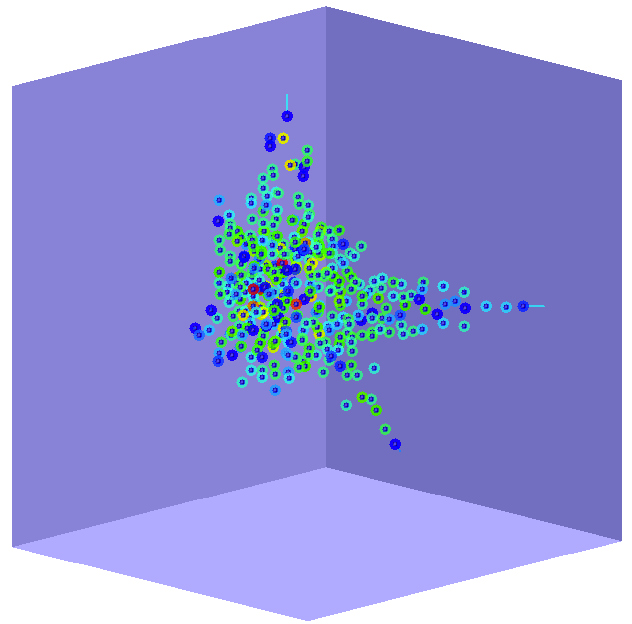
\includegraphics[width=0.95\textwidth]{\figpath/cascade.png} 


{\tiny \red{unfortunately the last pretty}}
\\ \vspace{-0.1in}
{\tiny \red{picture for today}}
\end{center}
\end{minipage}
}

%%%%%%%%%%%%%%%%%%%%%%%%%%%%%%%%%%%%%%%%%%%%%%%%%%%%%%%%%%%%%%%%%%%%%%%%%%%%
\section{\,}
%%%%%%%%%%%%%%%%%%%%%%%%%%%%%%%%%%%%%%%%%%%%%%%%%%%%%%%%%%%%%%%%%%%%%%%%%%%%

%\frame{\frametitle{Motivation}

%compositionally and structurally complex materials and processes: deposition (newtonian trajectory until hit) and radiation damage.

%}

%%%%%%%%%%%%%%%%%%%%%%%%%%%%%%%%%%%%%%%%%%%%%%%%%%%%%%%%%%%%%%%%%%%%%%%%%%%%
\section{Basic idea}
%%%%%%%%%%%%%%%%%%%%%%%%%%%%%%%%%%%%%%%%%%%%%%%%%%%%%%%%%%%%%%%%%%%%%%%%%%%%
\frame{\frametitle{Basic idea}

\vskip -0.1in

{\bf Premise:}
we can decompose the system into sub-configurations ({\it clusters}) \& if (isolated) sub-configurations are sufficiently large the forces on the central atoms are sufficiently accurate, \ie \blue{\bf locality}

\vskip 0.05in

\begin{minipage}{0.70\textwidth}
{\bf Procedure:}
\begin{enumerate}
\item
as dynamics ensues new ({\it query}) configurations are generated and compared to a cluster-force 
database.\item if sufficient stored clusters are close the query cluster the stored forces are interpolated at the query cluster   %   to those in the database the stored forces are used, perhaps using interpolation via radial basis functions
\item otherwise, {\it ab initio} forces are calculated for the new cluster and stored\end{enumerate}
\end{minipage}\hfill%
\begin{minipage}{0.29\textwidth}
{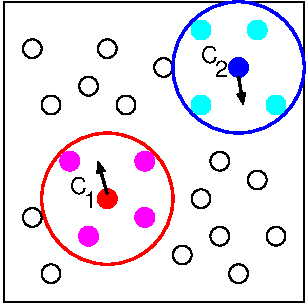
\includegraphics[width=1.0\textwidth]{\figpath/configuration.pdf}}
\end{minipage}

\vskip 0.05in

As opposed to the \red{\it globally}-tuned \red{\it empirical} potential, 
%we do not construct a compact surrogate potential energy function, 
we explicitly propogate the system in time using \red{\it locally interpolated} DFT forces. 

\vskip 0.05in

We endow the database with a distance measure that facilitates: (a) fast metric-based \blue{\bf searches} and (b) robust \blue{\bf interpolation} of database information at queries.

}
%%%%%%%%%%%%%%%%%%%%%%%%%%%%%%%%%%%%%%%%%%%%%%%%%%%%%%%%%%%%%%%%%%%%%%%%%%%%
\frame{\frametitle{Q1. Locality}
{\it Local} dependence of Hellman-Feynman force on configuration is the basic premise of all empirical potentials. 
{\bf Note: all data shown is from \abinitio molecular dyanmics}

\vspace{0.1in}

\begin{minipage}{0.55\textwidth}
Spatial decay of force due to a perturbation of Si 

\begin{center}
{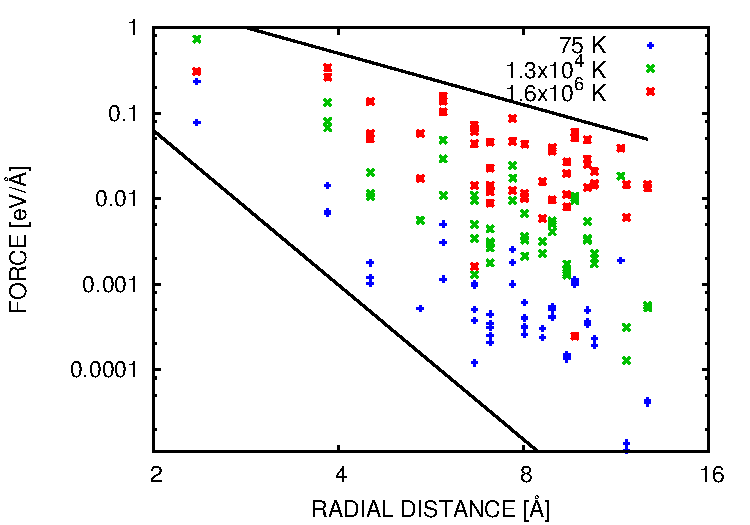
\includegraphics[width=0.9\textwidth]{\figpath/perturbation.pdf}}
\end{center}

Upper trend line is $\frac{1}{r^2}$, the lower  $\frac{1}{r^6}$.
Sensitive to disorder \& displacement
\end{minipage}\hfill\hspace{0.1in}%
\begin{minipage}{0.40\textwidth}
Convergence of the central atom force with cluster size.
\begin{center}
{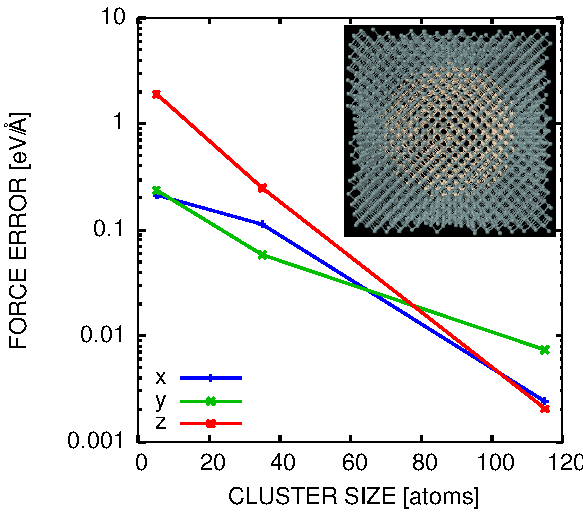
\includegraphics[width=0.9\textwidth]{\figpath/central_force_convergence.pdf}}
\end{center}

for a periodic 1000 atom C system \& spherical sub-configuration.
\end{minipage}
}

%%%%%%%%%%%%%%%%%%%%%%%%%%%%%%%%%%%%%%%%%%%%%%%%%%%%%%%%%%%%%%%%%%%%%%%%%%%%
\section{Algorithm}
%%%%%%%%%%%%%%%%%%%%%%%%%%%%%%%%%%%%%%%%%%%%%%%%%%%%%%%%%%%%%%%%%%%%%%%%%%%%
%%%%%%%%%%%%%%%%%%%%%%%%%%%%%%%%%%%%%%%%%%%%%%%%%%%%%%%%%%%%%%%%%%%%%%%%%%%%
\subsection{Distance metric}
%%%%%%%%%%%%%%%%%%%%%%%%%%%%%%%%%%%%%%%%%%%%%%%%%%%%%%%%%%%%%%%%%%%%%%%%%%%%

\frame{\frametitle{Cluster distance}
A {\it cluster} $\cluster_A$ is a set 
$
\cluster_A = \{ \dx_{1A}, \dx_{2A}, \dx_{3A}, \ldots, \dx_{N_A A} \}
$
of distance vectors 
$\Delta\xb_{\alpha A} \equiv \xb_\alpha - \xb_A$ 
relative to a central atom $\xb_A$,

\vspace{0.1in}
A distance $d(A,B)$ between clusters $\cluster_A$ \&  $\cluster_B$, needs
(a)
basic \blue{\bf metric} properties:
\begin{enumerate}
\item[M1] {\bf coincidence}:  $d(A,B) = 0 \ \text{iff} \ A=B $
\item[M2] {\bf positivity}:  $d(A,B) > 0 $
\item[M3] {\bf symmetry}: $d(A,B) = d(B,A)$
\item[M4] {\bf triangle inequality}: $d(A,C) \le d(A,B) + d(B,C)$
%\item[M5] {\bf reverse triangle inequality}: $d(A,C) \ge | d(A,B) - d(B,C) |$
\end{enumerate}

\vspace{0.1in}
and (b)  physical \blue{\bf invariances} $d(A,B) = d(A,B')$:
\begin{enumerate}
\item[II] {\bf translation} $\cluster_B \to \cluster_{B'} = \cluster_B + \ab$
\item[I2] {\bf rotation}    $\cluster_B \to \cluster_{B'} = \Rb \cluster_B $
\item[I3] {\bf permutation} $\cluster_B \to \cluster_{B'} = \Ps \cluster_B $
\end{enumerate}

}
%---------------------------------------------------------------------------
\frame{\frametitle{Root Mean Square Distance}

Assuming $N_A = N_B$, the root mean square deviation (RMSD) comparison metric is
\begin{equation*}
\begin{split}
d_\text{RSMD}(A,B) 
& %= \min_{\Rb,\Pb} d(\Xs_a, \Rb \Pb \Xs_b)
 = \min_{\Rb,\Ps} \| \Xs_A - \Ps \Xs_B \Rb^T \|  \\
%&= \min_{\Rb,\Ps} \sqrt{ \left( \Xs_A - \Ps \Xs_B \Rb \right) \cdot \Ws_{AB} \left( \Xs_A - \Ps \Xs_B \Rb^T \right) }
&= \min_{\Rb,\Ps} \sqrt{ \left( \Xs_A - \Ps \Xs_B \Rb^T \right) \cdot \Ws \left( \Xs_A - \Ps \Xs_B \Rb^T \right) }
 \\
&\equiv
\min_{\Rb,\Ps} \sqrt{ \sum_{\alpha,\beta=1}^{N_b} { \|\dx_{\alpha A} - \Ps_{\alpha\beta} \Rb \dx_{\beta B} \|^2  \
     \Ws_{\alpha \beta} } } %\negthinspace\left(( \| \dx_i)_a\|, \| (\dx_j)_b \| \right) }
\end{split}
\end{equation*}

\vskip -0.1in

where:\\
$\red{\bullet}$ $\Xs_A$ and $\Xs_B$ are matrices of the relative position vectors $\Delta \xb_\alpha$, 
\\
$\red{\bullet}$ $\Rb \in \mathsf{Orth^+}$ is a \underline{rotation} of the cluster \&
\\
$\red{\bullet}$ $\Ps$ is a \underline{permutation} of the cluster ordering, 
\ie a binary orthogonal matrix which is simply the rearrangement of the rows or columns of the identity matrix.

}

%---------------------------------------------------------------------------
\frame{\frametitle{Optimal rotation}

\vskip -0.2in 

\begin{equation*} 
\begin{split}
d(A,B) 
%&= \min_{\Rb,\Ps} \sqrt{ \left( \Xs_A - \Ps \Xs_B \Rb^T \right) \cdot \Ws_{AB} \left( \Xs_A - \Ps \Xs_B \Rb^T \right) } \\
%&= \min_{\Rb,\Pb} \sqrt{ \|\Xs_A\|^2_w + \|\Xs_B\|^2_w - 2 \Xs_A \cdot \Ws_{AB} \Ps \Xs_B \Rb^T }
&= \min_{\Rb,\Ps} \sqrt{ \left( \Xs_A - \Ps \Xs_B \Rb^T \right) \cdot \Ws \left( \Xs_A - \Ps \Xs_B \Rb^T \right) } \\
&= \min_{\Rb,\Pb} \sqrt{ \|\Xs_A\|^2 + \|\Xs_B\|^2 - 2 \Xs_A \cdot \Ws \Ps \Xs_B \Rb^T }
 \\
\end{split}
\end{equation*}
To determine the rotation $\Rb$, \slidecite{Kabsch}{}{1976} noticed the last term
\begin{equation*} 
2 \Xs_A \cdot \Ws \Ps \Xs_B \Rb^T
%= 2 \tr\left( \Ws(\Xs)\Rb \Pb \Xs_b \Xs_a^T\right)
%= 2 \tr\left( \Rb \Ps \Xs_B \Xs_A^T \Ws \right)
%= 2 \tr\left( \Xs_A \Rb ( \Ws \Ps \Xs_B)^T \right)
= 2 \Xs_A^T  \Ws \Ps \Xs_B \Rb^T
\end{equation*}
 is the only one dependent on $\Rb$.

\vskip 0.1in

A (3x3) singular value decomposition
$\SVD\left[ \Xs_A^T \Ws \Ps \Xs_B \right] = \Ub \Sb \Vb^T $
gives the solution $\Rb = \Ub \Vb^T$ and hence
\begin{equation*} 
d(A,B) = \min_{\Ps} \sqrt{ \|\Xs_A\|^2 + \|\Xs_B\|^2 - 2 \tr \Sb(\Ps)}
\end{equation*}
}

%---------------------------------------------------------------------------
\frame{\frametitle{Distance from Gaussian densities}
Finding the optimal \red{\it permutation} $\Ps$ is considerably harder, requiring \eg the $\mathcal{O}(n^3)$ Hungarian/branch \& bound algorithms.

\vskip 0.1in

Instead, the cluster atomic densities can be represented as an order-independent  sum of Gaussian smeared point {\bf densities}
\begin{equation*}
\rho(\xb) = \Delta(\mathbf{0}) + \sum_\alpha \Delta(\xb - \xb_\alpha) 
\end{equation*}

where \hspace{1.0in}
$
\Delta_\sigma(\xb) = \exp\left(- \frac{ \| \xb - \xb_\alpha \|^2}{2\sigma^2}\right) 
$

And hence
\begin{equation*}
d_\text{OGTO}(A,B) 
= \sqrt{\pi}^3 \sigma^3 \sum_{\alpha,\beta} \exp\left( -\frac{r_{\alpha\beta}^2}{4 \sigma^2} \right)
\end{equation*}

Finding the optimal rotation $\Rb$ and Gaussian width $\sigma$ is possible but the details are omitted here.

}
%---------------------------------------------------------------------------
\frame{\frametitle{Distribution of cluster distances}
%\centering
The distribution of inter-cluster distances as a function of:

\vspace{0.01in}

\begin{minipage}[h!]{0.4\textwidth}
 
{ \footnotesize
$\bullet$ {\bf metric}: RMSD \vs OGTO, 
the two metrics produce qualitatively different distributions 
\eg RMSD permutation sensitivity results in an artificial gap
}

\vspace{0.1in}


{ \footnotesize
$\bullet$ {\bf number of neighbors}: 4 (1st) \vs 16 (1st \& 2nd shells),
 more neighbors spreads the distance distribution \& is more discriminatory

\vspace{0.1in}

$\bullet$ {\bf temperature}: 300 K (crystalline) \vs 2500 K (melt),
both metrics indicate the expected structural changes with the shift from lattice to amorphous
}


\end{minipage}\hfill%
\begin{minipage}[h!]{0.55\textwidth}
\begin{center} 

{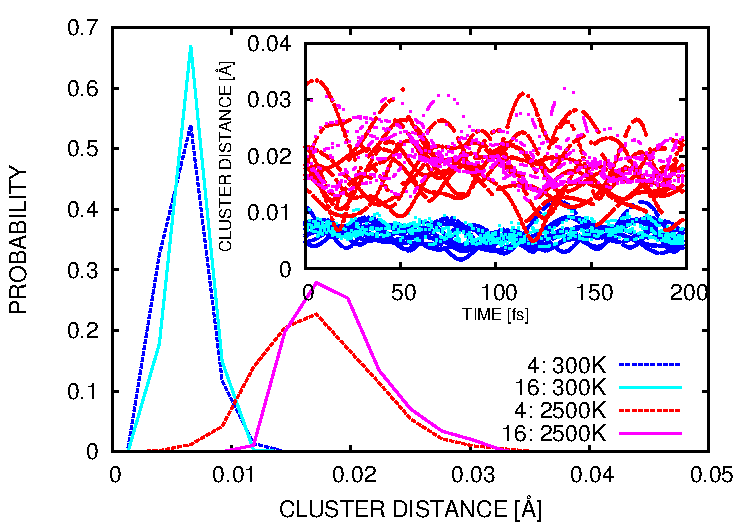
\includegraphics[width=0.85\textwidth]{\figpath/path_distribution.pdf}}

\hspace{0.2in}
$\Uparrow$ {\tiny single trajectory } \hspace{0.1in}
$\Downarrow$ {\tiny all atoms \& all times }

{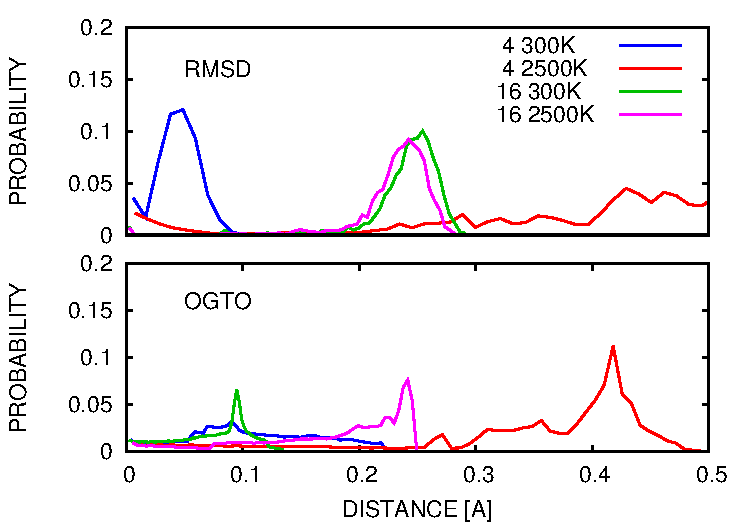
\includegraphics[width=0.95\textwidth]{\figpath/distribution.pdf}}

\end{center}
\end{minipage}

}

%%%%%%%%%%%%%%%%%%%%%%%%%%%%%%%%%%%%%%%%%%%%%%%%%%%%%%%%%%%%%%%%%%%%%%%%%%%%
\subsection{Metric search}
%%%%%%%%%%%%%%%%%%%%%%%%%%%%%%%%%%%%%%%%%%%%%%%%%%%%%%%%%%%%%%%%%%%%%%%%%%%%
%---------------------------------------------------------------------------
\frame{\frametitle{Metric database search}

\vskip -0.05in

A key ingredient is searching a large, dense database efficiently \slidecite{Fogolari}{}{2012} - utilize metric properties (M4)

\vskip -0.15in

\begin{minipage}[h!]{0.5\textwidth}
\fbox{
\begin{minipage}[h!]{0.99\textwidth}
\small
\begin{itemize}%[leftmargin=0pt]
%\setlength{\itemindent}{0em}
%\setlength{\listparindent}{0pt}
%\setlength{\leftmargin}{0pt}
\item {\bf Initialize:} \underline{\it select} a set of points $\{R_i\}$ in the database randomly or from previous time step.
%First set is random or uniformly sprinkled all subsequent sets are from history and cached in memory (and deleted if not used)
\item {\bf Loop:}
\begin{enumerate}
\item \underline{\it Find} closest in set:
$\argmin_{R}  d(Q,R_i)$, where Q is the query configuration 
%and $A_n$ is the nth point of the selected points.
%The point $A_m$ is the one with the smallest d(X, $A_m$).
\item \underline{\it Retrieve} neighboring set
$\{N\}$ of points about the point $R$  for which $2 d(N_i,R) < d(Q,R)$
\item \underline{\it Stop} if the neighborhood around $Q$ is the desired radius or size.
\end{enumerate}
\end{itemize}
\end{minipage}
}
\end{minipage}\hfill\hspace{0.1in}%
\begin{minipage}[h!]{0.45\textwidth}
{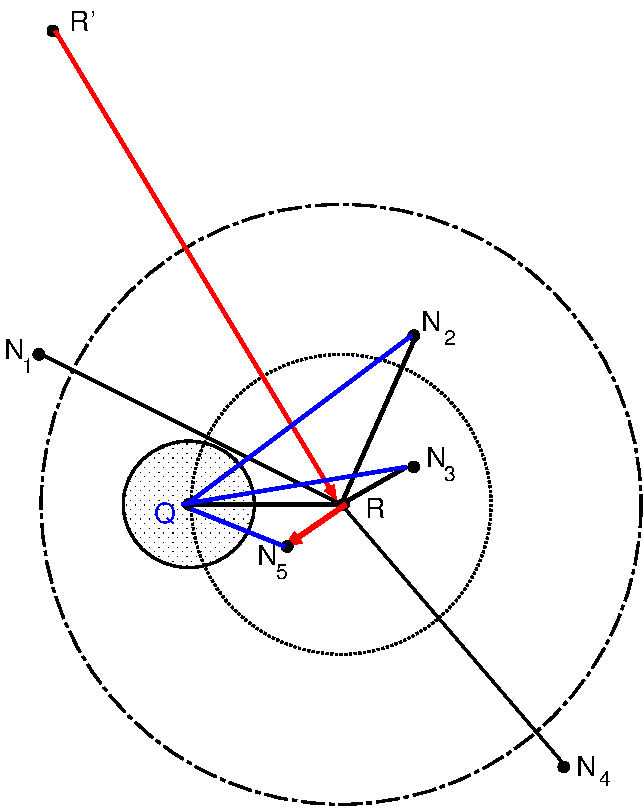
\includegraphics[width=0.9\textwidth]{\figpath/metric_search.pdf}}
{\tiny {\bf Query point} Q, {\bf reference point} R and its neighbors N$_i$ in the database. 
The subset \{  N$_2$, N$_3$, N$_5$ \} are candidates for configurations in the interpolation ball around Q. After computation of distances of the subset to Q, N$_5$ will be selected as the best candidate for the new R.}
\end{minipage}

}
%%%%%%%%%%%%%%%%%%%%%%%%%%%%%%%%%%%%%%%%%%%%%%%%%%%%%%%%%%%%%%%%%%%%%%%%%%%%
\subsection{Force interpolation}
%%%%%%%%%%%%%%%%%%%%%%%%%%%%%%%%%%%%%%%%%%%%%%%%%%%%%%%%%%%%%%%%%%%%%%%%%%%%
%---------------------------------------------------------------------------
\frame{\frametitle{Interpolation of forces}

\begin{minipage}[h!]{0.5\textwidth}
Given $\left\{d_{QN} \ | \ N \in \Ball_Q \right\}$, an accurate force $\fb_Q$ can be obtained from interpolation via {\bf radial basis functions} $\phi(r)$
\begin{equation*}
\fb_Q = \sum_{N\in \Ball_Q} \phi(d_{QN}) \, \ab_N 
\end{equation*}

where $\ab_N$ are given by the consistency conditions
\begin{equation*}
\Rb_{QN} \fb_N = \sum_{B\in \Ball_Q} \phi(d_{NB}) \, \ab_B  
\end{equation*}
for every $N \in \Bc_Q$


\end{minipage}\hfill%
\begin{minipage}[h!]{0.45\textwidth}
\begin{center}
{\bf Cluster space}

\vskip 0.1in

{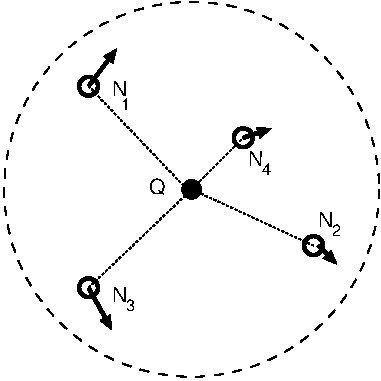
\includegraphics[width=0.99\textwidth]{\figpath/interpolation_schematic.pdf}}

\vskip 0.1in

{\small this is the (shaded) trust ball around the query point Q in the previous slide}
\end{center}
\end{minipage}
}

%%%%%%%%%%%%%%%%%%%%%%%%%%%%%%%%%%%%%%%%%%%%%%%%%%%%%%%%%%%%%%%%%%%%%%%%%%%%
\section{Results}
%%%%%%%%%%%%%%%%%%%%%%%%%%%%%%%%%%%%%%%%%%%%%%%%%%%%%%%%%%%%%%%%%%%%%%%%%%%%
%---------------------------------------------------------------------------
\frame{\frametitle{Questions}

\begin{minipage}[h!]{0.55\textwidth}
The algorithm is viable if:
\begin{itemize}
\item[\black{\bf Q1.}] \black{{\bf sensitivity} of the forces to the configuration is {\bf local}}
\item[{\bf Q2.}] \blue{inter-cluster {\bf distances} are {\bf correlated} with {\bf forces} on the central atoms}
\item[{\bf Q3.}] \blue{the search is sufficiently {\bf efficient}}
\item[{\bf Q4.}] \blue{the {\bf error} in interpolating the force is {\bf controllable}}
\end{itemize}
\end{minipage}%
\begin{minipage}[h!]{0.44\textwidth}
{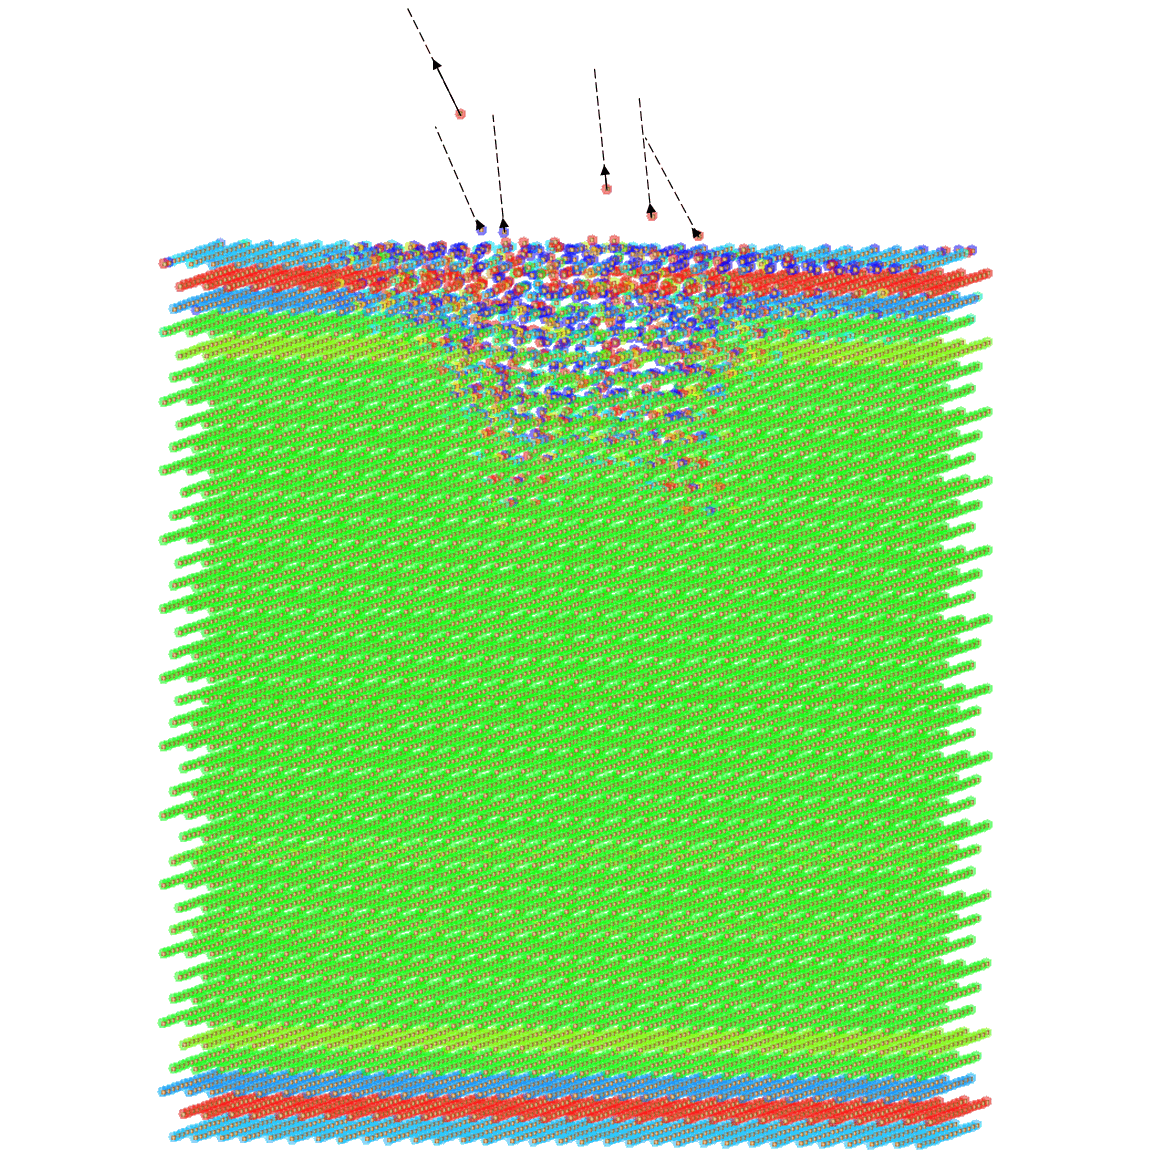
\includegraphics[width=1.25\textwidth]{\figpath/sputter.png}}
\vspace{0.2in}
\end{minipage}
}
%---------------------------------------------------------------------------
\frame{\frametitle{Q2. Correlation of cluster distance and forces}
The difference in forces on the central atom for two clusters

\vskip 0.05in

\begin{minipage}[h!]{0.38\textwidth}

$$\| \fb_A - \fb_B \| \propto d(A,B)$$

\vskip 0.1in

is highly \& linearly correlated with the inter-cluster distance $d(A,B)$.

\vspace{0.1in}

The correlation is dependent on temperature and less so on number of neighbors.


\end{minipage}\hfill%
\begin{minipage}[h!]{0.6\textwidth}
\begin{center} 

%{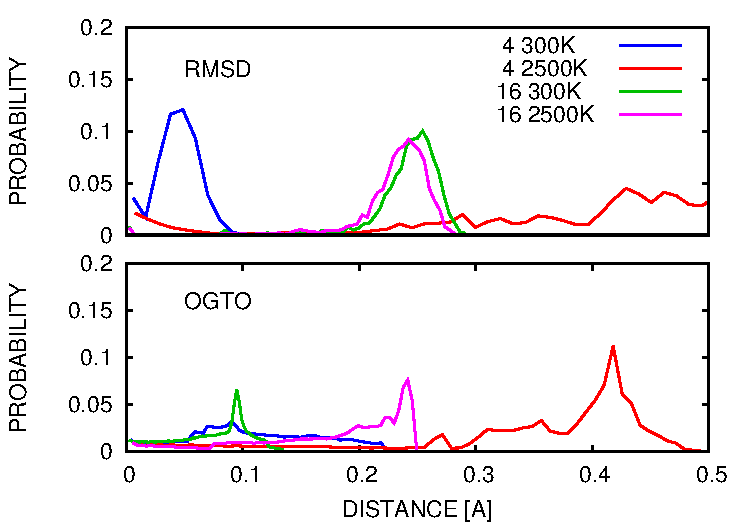
\includegraphics[width=0.95\textwidth]{\figpath/distribution.pdf}}


{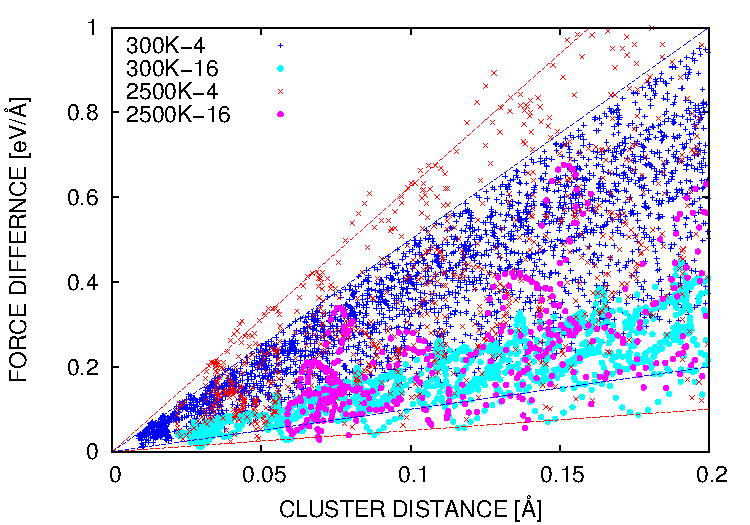
\includegraphics[width=0.95\textwidth]{\figpath/OGTO_force-distance_correlation.pdf}}

{\bf $\Longleftarrow$ better match}
\end{center}

\end{minipage}

\begin{center}
The sensitivity is $\approx$ 10 eV/\AA$^2$
\end{center}
}
%---------------------------------------------------------------------------
\frame{\frametitle{Q3. Metric search efficiency}

\vskip -0.05in

Measuring search efficiency as: $\displaystyle\frac{d}{s}$ 

\hspace{0.1in} where $s$=database size \& $d$=number of distance computations 

\vskip 0.05in


\vskip -0.1in

\begin{center}
{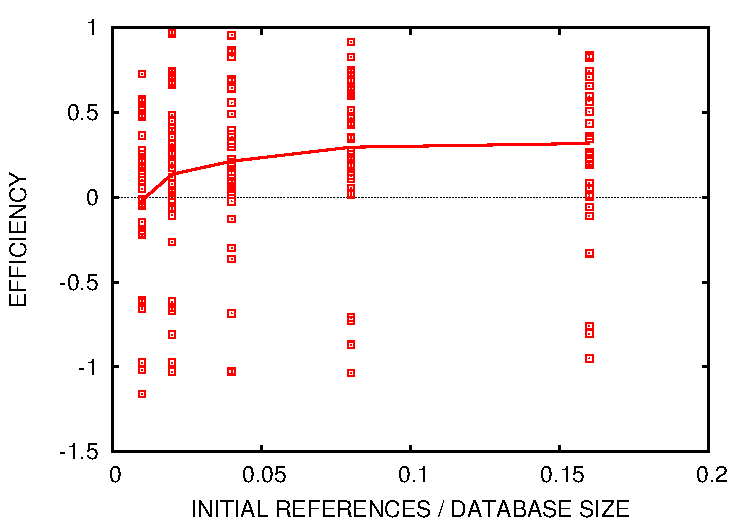
\includegraphics[width=0.65\textwidth]{\figpath/metric_search_efficiency.pdf}}
\end{center}

%\vskip -0.1in


This is a worst-case for dynamics, subsequent steps would use the previous as a starting guess.

%As the number of initial {\it reference} clusters, clusters chosen for \underline{new} calculations of distance to the query cluster, increases the metric search becomes more efficient. 
%This trend has a obvious limit as the entire database is sampled by the initial set of reference clusters
}


%---------------------------------------------------------------------------
\frame{\frametitle{Q4. Force interpolation error}

Measuring interpolation of error as $\displaystyle\frac{\| \hat\fb - \fb \|}{\| \fb \|}$ 
\begin{center}
{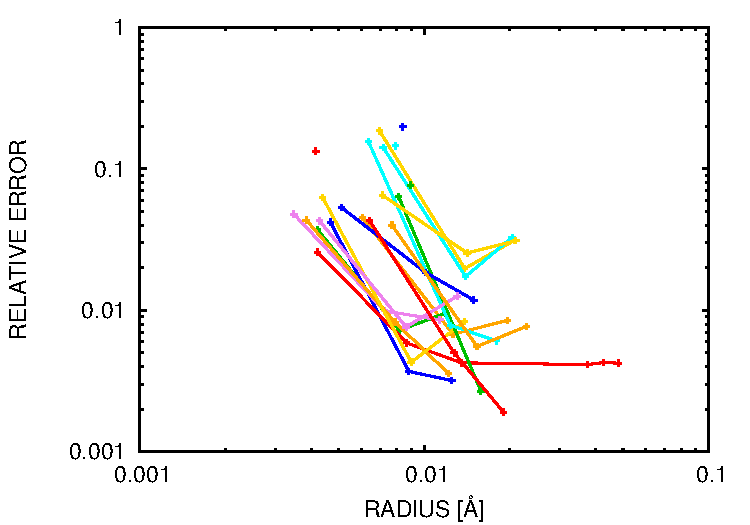
\includegraphics[width=0.65\textwidth]{\figpath/force_error.pdf}}
\end{center}

where $\fb$=true force  \& $\hat\fb$=interpolated force (not using the true force sample)  and $R$ is the radius of the trust ball in cluster space
}

%---------------------------------------------------------------------------
\frame{\frametitle{Conservation properties}

Momentum and temperature as a function of time:

\begin{center}
{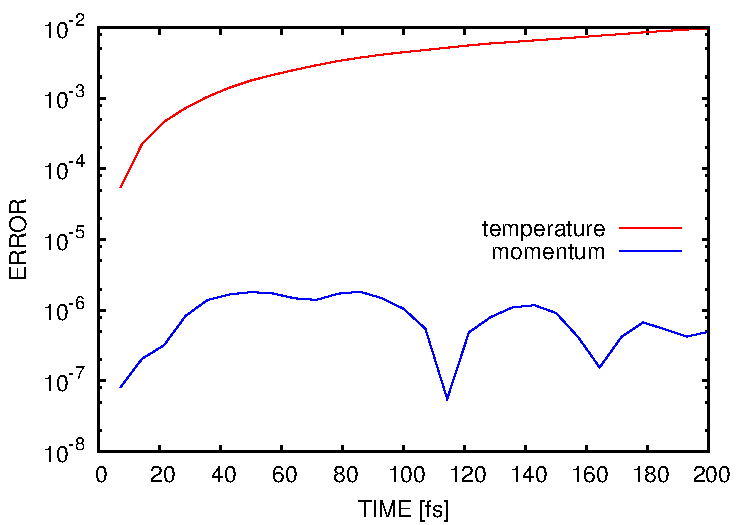
\includegraphics[width=0.65\textwidth]{\figpath/dynamics_error.pdf}}
\end{center}

\vskip -0.1in

we don't have a direct means of measuring potential energy.

\vskip 0.1in

We can control temperature with a thermostat.

}

%%%%%%%%%%%%%%%%%%%%%%%%%%%%%%%%%%%%%%%%%%%%%%%%%%%%%%%%%%%%%%%%%%%%%%%%%%%%
\section{Conclusion}
%%%%%%%%%%%%%%%%%%%%%%%%%%%%%%%%%%%%%%%%%%%%%%%%%%%%%%%%%%%%%%%%%%%%%%%%%%%%
{
\usebackgroundtemplate{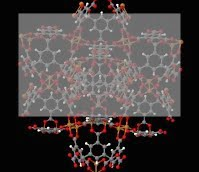
\includegraphics[width=\paperwidth]{\figpath/backgroundMOF.jpg}}%
\frame{\frametitle{\textcolor{yellow}{Current work}}

\vskip 0.2in

%\transparent{0.9}\colorbox{white}{
\begin{minipage}[h!]{\textwidth}
\begin{itemize} \setlength{\itemsep}{0.2in}
%\item \green{We have results for the dynamics of  1- and 3-D test systems but they are aren't that interesting since we have only been testing consistency of the method and full \abinitio and classical molecular dynamics.}

\item  \green{ Application to atomic deposition, radiation damage, and structurally interesting materials like metal-organic frameworks is upcoming.}

\item \green{Since the method reduces to {\it ab initio} molecular dynamics in the limit to full system clusters and no interpolation, we are trying to make stronger connections to it.}

\item \green{We are also exploring using machine learning techniques to enhance the search and interpolation methodology. }
\end{itemize}
\end{minipage}
%}

\vskip -0.2in

\begin{center}
\colorbox{yellow}{
{Reese Jones} \blue{\bf rjones@sandia.gov}
}
\end{center}
}

\end{document}
